%--------------------------------------------------------
%--------------------------------------------------------
\section{Generalized operators}
The azimuthal of the convolution kernel $\mathcal{M}$ could have been been argued to have the form $e^{-i2 \alpha}$ by requiring to construct a spin-0 field given some spin-2 fields. In this sense there is no freedom in the choice of the azimuthal dependence of the convolution kernels. The radial part of this kernel however is determined by the basis functions. It is possible to generalize these convolution kernels by choosing alternate forms for the radial functions, without affecting the parity properties of the scalar fields $E$ \& $B$.

We can characterize different forms of the radial kernel by introducing the following harmonic space operator,
%
\beq
\tilde{\mathcal{G}} = {\begin{bmatrix} g_{\ell}^E & 0  \\  0 & g_{\ell}^B \end{bmatrix}} \,,
\eeq
%
where the functions $g_{\ell}^E$ and $g_{\ell}^B$ represent the harmonic representation of the modified radial functions and can in the most general case be chosen to be different for $E$ and $B$ modes. To simplify the discussion and without loosing generality we proceed by setting $g_{\ell}^E = g_{\ell}^B= g_{\ell}$. Once we have made a choice for these harmonic functions, we can define the real space operator $\bar{O}'$ which translates Stokes $Q$ \& $U$ to scalars $E$ \& $B$ and the inverse operator $\bar{O}'^{-1}$ in the following manner,
%
\begin{subequations} \label{eq:gen_qu2eb}
\beqry
{\bar O}' &=& {{}_0\mathcal{Y}} *\tilde T^{-1}*\tilde{\mathcal{G}}* {{}_2\mathcal{Y}^{\dagger}} *\bar T \,,\\
{\bar O}'^{-1}&=& \bar{T}^{-1} *{{}_2\mathcal{Y}}* \tilde{\mathcal{G}}^{-1} *\tilde T *{{}_0\mathcal{Y}^{\dagger}}
\eeqry
\end{subequations}
%
where we have used the primed notation  to distinguish these generalized operators from the default operators defined in \sec{sec:qu2eb} and \sec{sec:eb2qu}. Note that for an arbitrary choice of $\tilde{\mathcal{G}}$ only one of the operators in \eq{eq:gen_qu2eb} is well defined, since $\tilde{\mathcal{G}}^{-1}$ may be ill defined. If we require both the forward and inverse operators to be well defined, then we are constrained in choosing $\tilde{\mathcal{G}}$ such that it has a valid  inverse. As we will see this will be an important criteria to recover the standard CMB spectra. The radial part of these generalized convolution kernels is given by the following expressions,
%
\begin{subequations}
\beqry
G_{QU \rightarrow EB}(\beta) &=& G(\beta) = \sum _{\ell=2} ^{\ell_{\rm max}} g_{\ell}\frac{2 \ell+1}{4 \pi} \sqrt{\frac{(\ell-2)!}{(\ell + 2)!}} P_{\ell}^2(\cos{\beta}) \, \label{eq:mod_rad_forward} \\
G_{EB \rightarrow QU}(\beta) &=& G^{-1}(\beta) = \sum _{\ell=2} ^{\ell_{\rm max}} g_{\ell}^{-1}\frac{2 \ell+1}{4 \pi} \sqrt{\frac{(\ell-2)!}{(\ell + 2)!}} P_{\ell}^2(\cos{\beta}) \,,\label{eq:mod_rad_inverse}
\eeqry
\end{subequations}
%
where $g_{\ell}$ are the same multipole function as those appearing in $\tilde{\mathcal{G}}$. Given this general definition for the radial function $G(\beta)$, note that the default radial function ${{}_{\mm}f}$ is just a special case resulting from the choice $\tilde{\mathcal{G}}=\mathbb{1}$ ($g_{\ell}=1$). Note that for this choice of $\tilde{\mathcal{G}}$ the inverse is trivial $\tilde{\mathcal{G}}^{-1}=\tilde{\mathcal{G}}$ and therefore $G^{-1}(\beta) = G(\beta)$.

While defining these generalized operators, it seems more natural to choose the real space function $G(\beta)$ as compared to choosing the multipole function $g_{\ell}$. Using the orthogonality property of associated Legendre polynomials it can be shown that the harmonic function $g_{\ell}$ is given by the following integral over the radial function $G(\beta)$,
%
\beq
g_{\ell} = 2 \pi \sqrt{\frac{(\ell-2)!}{(\ell+2)!}} \int _{0}^{\pi} G(\beta) P_{\ell}^{2}(\cos{\beta}) d\cos{\beta} \,. \label{eq:gb2bl}
\eeq
%
To ensure that the resultant field is a spin-0 field, it is important to note that the radial function $G(\beta)$ has to be necessarily chosen such that it vanishes at $\beta=0$ and $\beta=\pi$. 
%One way to understand this is that the associated Legendre polynomials $P_{\ell}^2 \propto \sin^2{\beta}$ vanish at these values of the abscissa and hence cannot be used to describe functions which don't have this property.  Another way to understand this requirements is that at these locations the coordinate dependence of the Stokes parameters cannot be integrated out, since the azimuthal angle is ill defined and hence the convolution kernel needs to have vanishing contribution from these locations. \revisit{The normalization of these functions is not critically important, since any choice defines a convention. It is important to ensure consistency with the convention once a choice has been made.} \comment{find a better location for this}

An arbirtrary $G(\beta)$ for which $g_{\ell} \neq 1$ can be equivalently thought in terms of the standard E and B mode fields being convolved with some circularly symmetric instrument beam. 
Note that in contrast to the radial function $G(\beta)$ an instrumental beam function appropriately normalized has the property $B(\beta) \rightarrow 1$ as $\beta \rightarrow 0$. We clarify that the $B(\beta)$ refers to the effective beam acting to smooth the scalar $E$ \& $B$ mode maps. A circularly symmetric beam $B(\beta)$ defined at the pole can be expressed in the Legendre polynomial $P_{\ell}^0$ basis as follows,
%
\beq
B(\beta) = \sum_{\ell=0}^{\ell_{\rm max}} \frac{2 \ell+1}{4 \pi} b_{\ell} P_{\ell}^{0} (\cos{\beta})\,,
\eeq
%
where $b_{\ell}$ denote the coefficients of expansion. \comment{Note that one can directly get E and B mode maps resulting from convolution with a non-circular beam by chosing the function $g_{\ell}$ to have some m dependence.}
%
\begin{figure}[!t] 
\centering
\subfigure[\label{fig:bl_gbeta}]{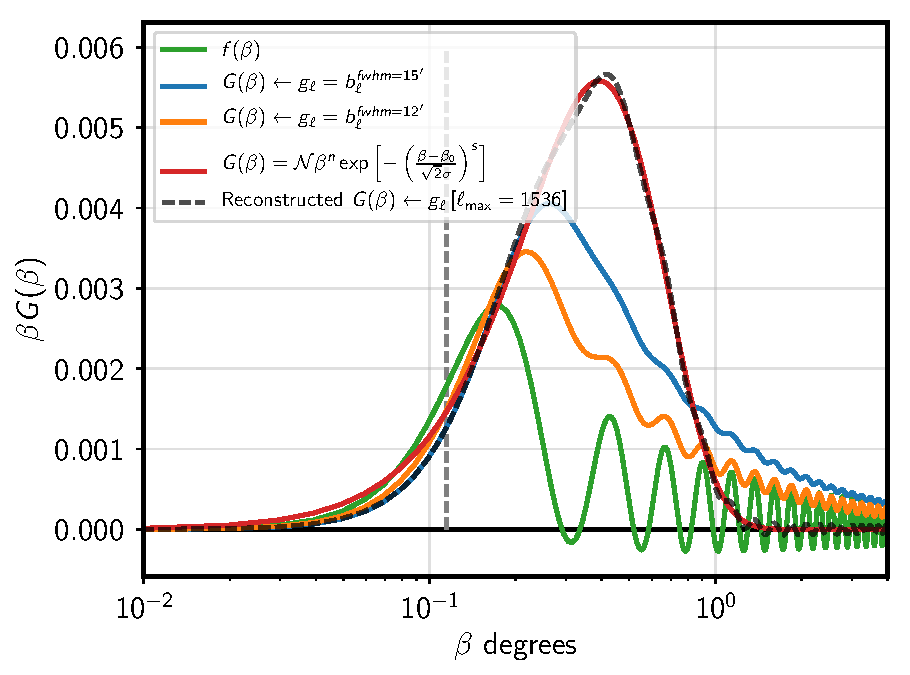
\includegraphics[width=0.48\columnwidth]{Gbeta_for_different_gl_lmax1536.pdf}}
\subfigure[\label{fig:glbl}]{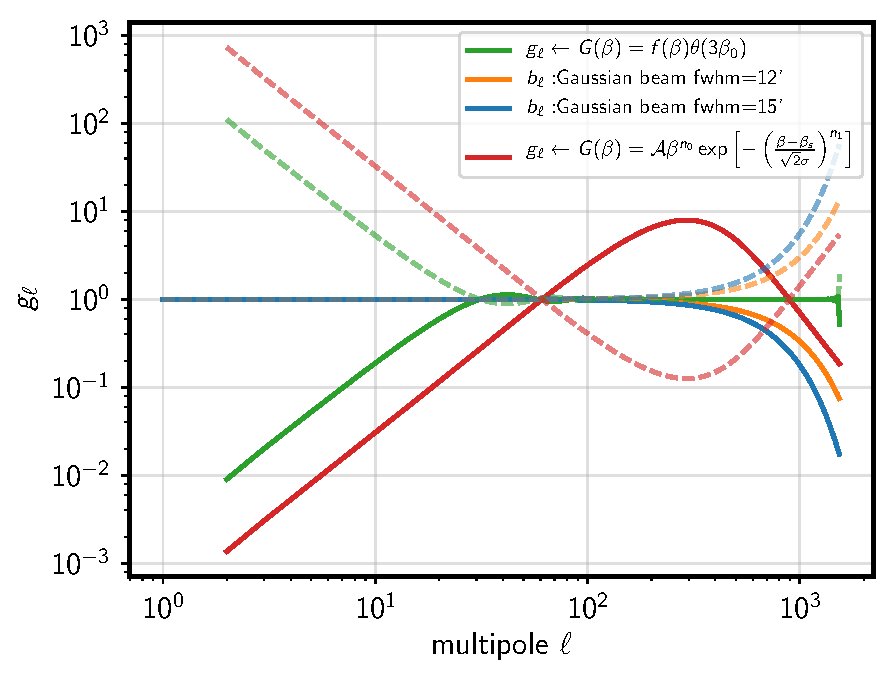
\includegraphics[width=0.48\columnwidth]{gl_for_different_gbeta_lmax1536.pdf}}
\subfigure[\label{fig:gl_bbeta}]{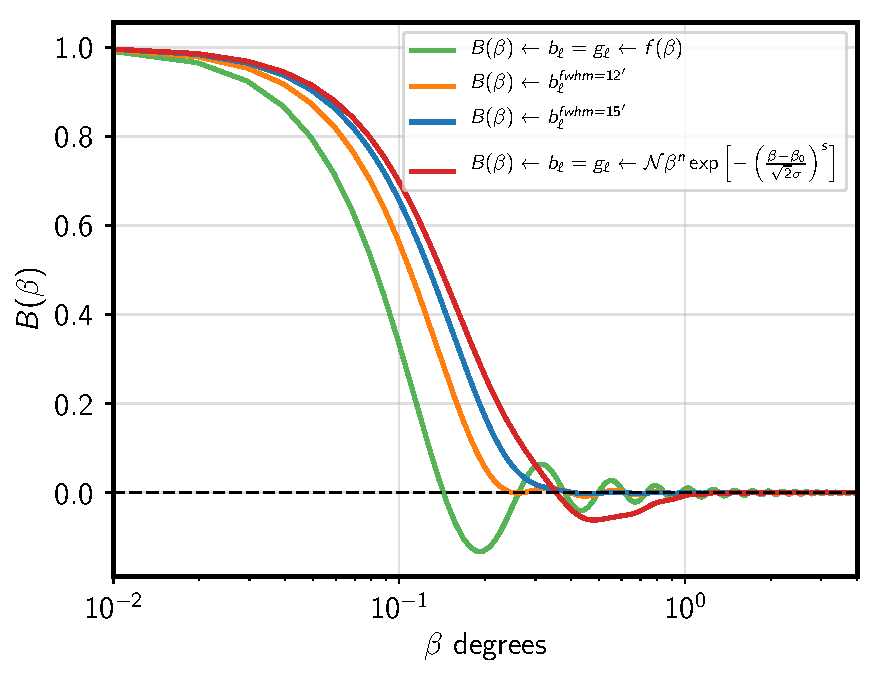
\includegraphics[width=0.48\columnwidth]{Bbeta_for_gl_lmax1536.pdf}}
\caption{\textit{Left:} The vertical dashed gray line depicts the approximate pixel size $\Delta_{\rm pix} = \sqrt{\frac{4 \pi}{N_{\rm pix}}}$ of a Nside=512 Healpix map. The green line depicts the default radial kernel $f(\beta)$ defined in \eq{eq:qu2eb_gen_kernel}. The blue and orange lines depict the modified radial function resulting the beam harmonics $b_{\ell}$ corresponding to Gaussian beams with fwhm=15 \& 12 arcminutes respectively. The red curve depicts an example modified radial function: $G(\beta)=\mathcal{N} \beta^n \exp{\left[ -\left( \frac{\beta-\beta0}{\sqrt{2} \sigma} \right)^s \right]}$ with parameters set to the following values $[n=1;\, \beta_0=0 ;\, \sigma = 2\Delta_{\rm pix} ;\, s=1.5]$. The black dashed curve depicts the band limited reconstruction of the modified radial function $G(\beta)$. We intentionally have plotted $\beta G(\beta)$ to clearly depict the high $\beta$ behavior of these functions. \textit{Middle: } This figure depicts the harmonic representation of the respective radial functions as indicated by the legend. The dashed curves of the corresponding color depict the inverse of the harmonic functions. \textit{Right:} This figure depicts the beam function $B(\beta)$ evaluated from interpreting the respective harmonic functions as those corresponding to an instrument beam.}
\label{fig:example_gbeta}
\end{figure}
%

Though the real space behavior of these two function $G(\beta)$ and $B(\beta)$ has important differences, in harmonic space they play identical roles. Therefore it is possible to interpret the beam harmonic coefficients as those representing some modified radial kernel. \fig{fig:glbl} depicts the harmonic functions $g_{\ell} (b_{\ell})$ for the respective radial kernel and beams.  The modified radial kernel resulting from Gaussian beams with ${\rm fwhm} =15' \,\&\, 12'$ are depicted in \fig{fig:bl_gbeta} as blue and orange curves respectively. Note that instruments  beams tend to increase the non-locality parameter $\beta_0$, indicated by the shifting right of the maxima of the respective kernels, as one may have expected. The red curve depicts a modified radial kernel which by construction has a very small $\beta_0$.  Similarly it is possible to interpret the harmonic representation $g_{\ell}$ of the radial function $G(\beta)$ as those corresponding to some instrument beam function. The beam function corresponding to the default radial kernel ($g_{\ell}=1$) is merely a band limited representation of the delta function depicted by the green curve \fig{fig:gl_bbeta}, while the red curve depicts the same for the modified radial kernel.

%In \sec{sec:local_conv_eb} we constructed localized convolution kernels by multiplying $R(\beta)$ with an apodized version of the step function $\theta_{\rm apo}(r_{\rm cutoff})$. The oscillation seen in the spectra in \fig{fig:eb-spectra_rad_cutoff} can be explained to be due to this effective beam characterized by $g_{\ell}^2$ operating on the power spectra. The effective beam can be evaluated by computing the multipole function $g_{\ell}$ as follows,
%%
%\beq
%g_{\ell} = 2 \pi \sqrt{\frac{(\ell-2)!}{(\ell+2)!}} \int _{0}^{r_{\rm cutoff}} R(\beta) \theta_{\rm apo}(r_{\rm cutoff})  P_{\ell}^{2}(\cos{\beta}) d\cos{\beta} \,, \label{eq:gb2bl} \,,
%\eeq
%%
%where the upper limit of the integration is set to $r_{\rm cutoff}$ since the function $\theta_{\rm apo}(r_{\rm cutoff})$ vanishes for $\beta>r_{\rm cutoff}$. The function $b^2_{\ell}-1$ matches the oscillation seen in \fig{fig:eb-spectra_rad_cutoff} as  seen in \fig{fig:match_cl_oscillations} where the two results have been over plotted.
%%
%\begin{figure}[!t] 
%\centering
%\subfigure[]{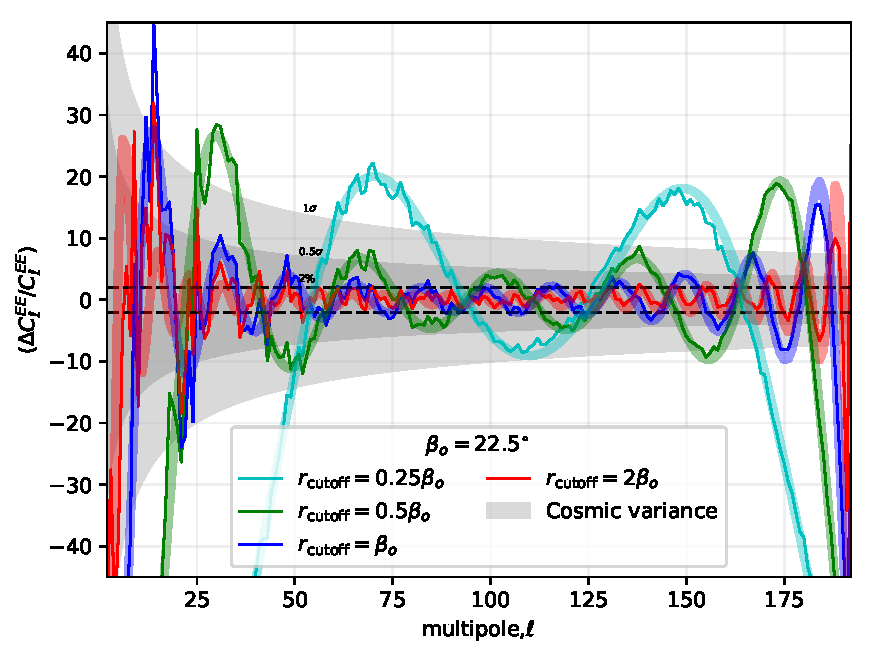
\includegraphics[width=0.98\columnwidth]{analytical_cl_oscillations_vs_data.pdf}}
%\caption{The thin lines depicts the same spectral differences as those seen in \fig{fig:eb-spectra_rad_cutoff}, while the thick lines of the corresponding color depict the function $g_{\ell}^2 -1$ as derived from evaluating \eq{eq:gb2bl} for different $r_{\rm cutoff}$}.
%\label{fig:match_cl_oscillations}
%\end{figure}
%%
%The apodized step function in this case transition from 1 at $\beta < r_{\rm cutoff} -w$ to 0 at $r_{\rm cutoff}$ over a width $w= 3^{\circ}$ with a cosine squared profile .

\subsection{Recovering the default $E$ and $B$ mode spectra}
The generalized convolution kernels defined in the previous section, when operated on the Stokes vector returns some scalar $E'$ and $B'$ mode maps,
%
\beq
\bar{S}' = \bar{O}' * \bar{P}
\eeq
%
which as we show are mere filtered version of he standard $E$ and $B$ modes maps. The harmonic representation $g_{\ell}$ of the radial function $G(\beta)$ can be simply interpreted as the harmonic coefficients of some azimuthally symmetric beam $B(\beta) = \sum_{\ell} \frac{2 \ell+1}{4 \pi} g_{\ell} P^0_{\ell}(\cos{\beta})$. The spectra of the scalar fields $E'$ and $B'$ derived using the real space operators constructed using an arbitrary radial function $G(\beta)$ are related to the spectra of the standard $E$ and $B$ fields via the following relation, 
 %
 \begin{subequations}
 \beqry
C_{\ell}^{EE,BB,EB} &= &C_{\ell}^{E'E',B'B',E'B'} /   g_{\ell}^2\,,\\
C_{\ell}^{TE,TB}  &=&  C_{\ell}^{TE',TB'} / g_{\ell}\,,
 \eeqry
 \end{subequations}
 %
 where $C_{\ell}$ denotes the angular power spectra and $T$ refers to the temperature anisotropy map. Therefore the standard $E$ and $B$ mode spectra can be recovered from the modified fields $E'$ and $B'$ and their accurate recovery only relies on the inverse of the harmonic functions $1/g_{\ell}$ being well behaved, which can be ensured by making a suitable choice for the radial function $G(\beta)$. Examples of various forms of $G(\beta)$, its harmonic representation $g_{\ell}$ (and its inverse $1/g_{\ell}$ ) and the corresponding beam $B(\beta)$ are depicted in \fig{fig:example_gbeta}.
%One direct application of this freedom in choosing the radial kernel is that one can mitigate the issue of leakage of power from $E$ to $B$.  By constructing a radial function which tapers to zero at sufficiently small radii one can clearly discard pixels which are affected by masking. 
%--------------------------------------------------------
%--------------------------------------------------------
